\chapter{Grundlagen}
\achtung{\textbf{Wichtig} FAS bitte nur \textbf{einmal} �ffnen!\\
	Gleichzeitiges Arbeiten mit mehreren Instanzen von FASonline kann zu Aktualisierungsproblemen bei Semesterwechseln f�hren.}\\

\section{Aufbau der Arbeitsoberfl�che}
\begin{figure}
	\begin{center}
    \begin{picture}(128,89)
			\put(0,0){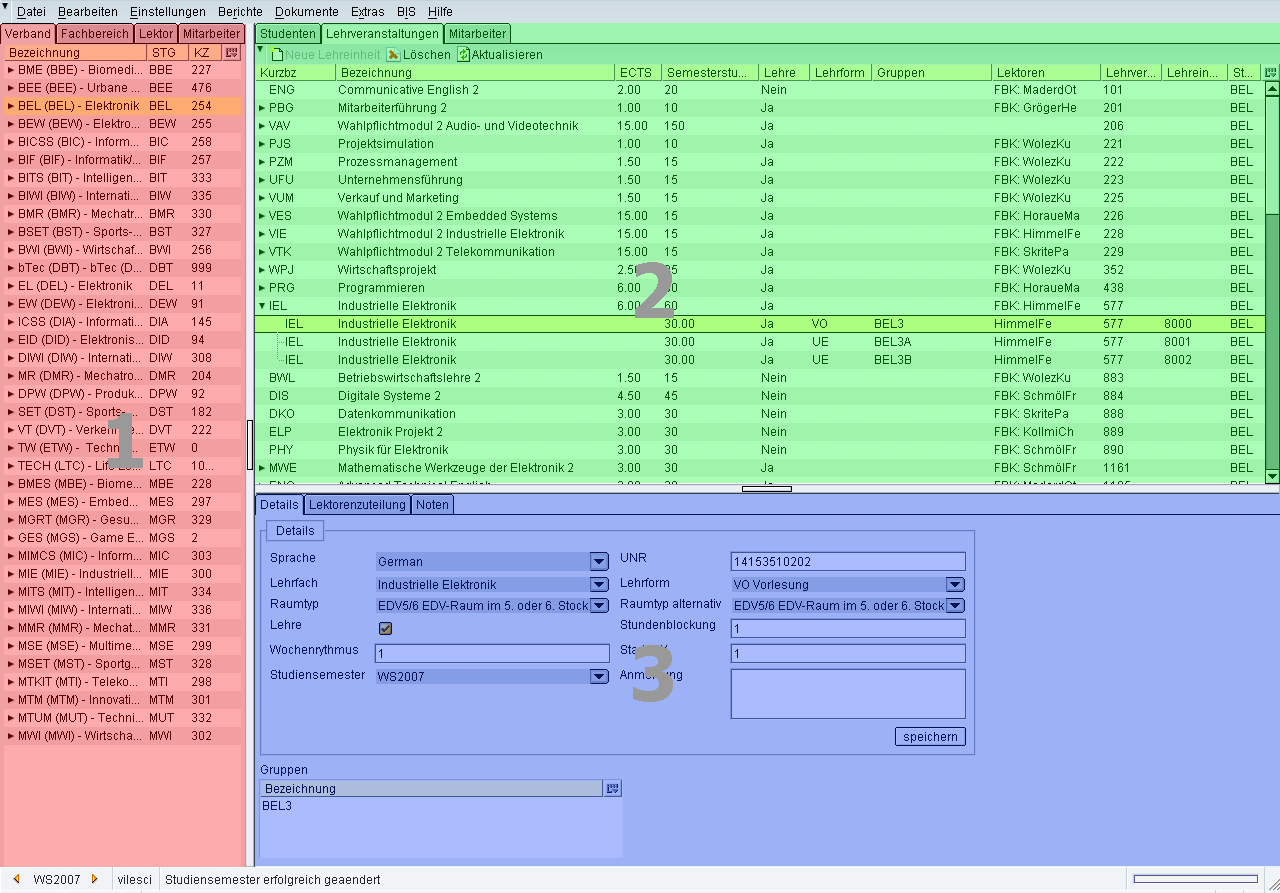
\includegraphics[height=89mm, width=128mm]{FAS_Grundlagen1.png}}
			\markier{4}{6}{8}{0}{-1}
			\markier{5}{20}{8}{-1}{-1}
		\end{picture}
    \caption{Aufbau der Oberfl�che}
		\label{Grundlagen1}
  \end{center}
\end{figure}
\subsection{Listenfeld 1}
\begin{itemize}
	\item Verband: In dieser Karteikarte werden nur die Studieng�nge angezeigt, f�r die der Anwender Zugriffsrechte besitzt. Wenn es zu einer Zeile Untergruppierungen gibt, wird links neben dem Namen ein Symbol angezeigt. Abbildung \ref{Grundlagen2} zeigt den strukturellen Aufbau eines Studiengangs. 
\begin{figure}
	\centering
	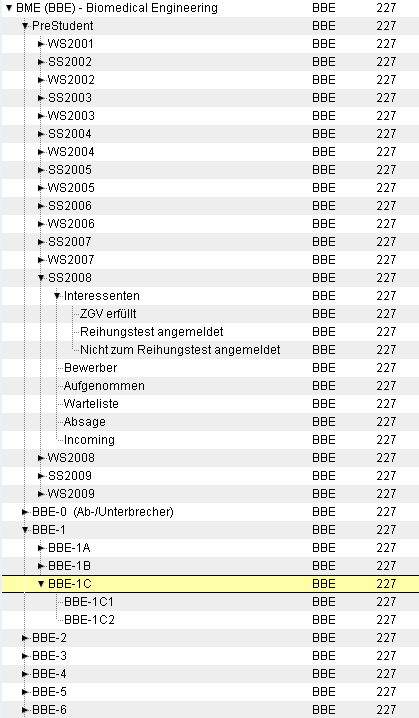
\includegraphics[width=0.55\textwidth]{FAS_Grundlagen2.png}
	\caption{Anzeige Stundiengang}
	\label{Grundlagen2}
\end{figure}
		\begin{itemize}
			\item Prestudent: 
			Als Prestudent werden alle Personen bezeichnet die noch keine Studenten sind (\textsl{pre}(lat.) - \textsl{vor}). Die Aufteilung der Prestudenten erfolgt in Semester und da dann noch in verschiedene Interessenten sowie Bewerber, Aufgenommene, Personen auf der Warteliste und Personen die abgesagt haben bzw. denen abgesagt wurde.
			Weiters finden sich hier die Incoming \underline{aller} Studieng�nge dieses Semesters.
			\item Semester: Es werden immer alle Semester mit Lehrverb�nden und Gruppen angezeigt, auch die in diesem Semester nicht aktiven. 
		\end{itemize}
	\item Institut: Zur Anzeige der Institutsliste mu� nach �ffnen der Karteikarte die Taste 
\includegraphics{icon_aktualisieren} angeklickt werden. Die Liste z�hlt die Institute und die zugeordneten Lektoren auf. Markiert man einen Lektor erscheinen im Listenfeld 2 alle Lehrveranstaltungen dieses Fachbereichs, in denen dieser Lektor unterrichtet. 
	\item Lektor: Alle Lektoren auch zugeteilt zu Studieng�ngen.
	\item Mitarbeiter: Mehrere Listenansichten dem Mitarbeiter gefiltert nach den in Abbildung \ref{Grundlagen3} gezeigten Kriterien. Die Anzeige der Lektoren erfolgt in Listenfeld 2.
	\begin{figure}
		\centering
		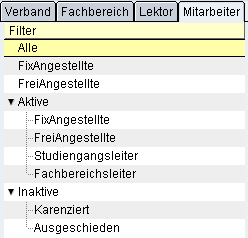
\includegraphics[width=0.55\textwidth]{FAS_Grundlagen3.png}
		\caption{Anzeige Mitarbeiter}
		\label{Grundlagen3}
	\end{figure} 
\end{itemize}
\subsection{Listenfeld 2}
\begin{itemize}
	\item Studenten: Liste von Studenten, gefiltert nach der Auswahl in Listenfeld 1 oder einer Suche.
	\item Lehrveranstaltungen: Liste von Lehrveranstaltungen mit zugeordneten Lehreinheiten, gefiltert nach Auswahl in Listenfeld 1.
	\item Mitarbeiter: Anzeige von Mitarbeiter, gefiltert nach der Auswahl von Listenfeld 1.
\end{itemize}
\subsection{Datenbereich}
Die Anzeige in diesem Teil ist von der Auswahl im Listenfeld 2 abh�ngig und zeigt Detaildaten an bzw. k�nnen diese hier eingegeben und ge�ndert werden.\\
Bei Auswahl in Listenfeld 2 zeigt der Datenbereich folgende Karteikarten:
\begin{itemize}
	\item Studenten: 	
	\begin{itemize}
		\item Details - Kapitel \ref{details}
		\item Kontakt - Kapitel \ref{kontakte}
		\item PreStudent - Kapitel \ref {prestudent}
		\item Dokumente - Kapitel \ref{dokumente}
		\item Konto - Kapitel \ref{studentenkonto}
		\item Betriebsmittel - Kapitel \ref{betriebsmittel}
		\item In/Out - Kapitel \ref{Incoming} und \ref{Outgoing}
		\item Noten - Kapitel \ref{noten}
		\item Zeugnis - Kapitel \ref{zeugnis}
		\item Pr�fung - Kapitel \ref{pruefungen}
		\item AbschlussPr�fung - Kapitel \ref{abschlusspruefungen}
		\item Projektarbeit - Kapitel \ref{projektarbeit}
		\item Gruppen - Kapitel \ref{gruppen}
		\item Funktionen - Kapitel \ref{funktionen}
	\end{itemize}
	\item Lehrveranstaltungen - Kapitel \ref{lehrveranstaltung}: 
	\begin{itemize}
		\item Details 
		\item Lektorenzuteilung 
		\item Noten
	\end{itemize}
	\item Mitarbeiter - Kapitel \ref{mitarbeiter}:
	\begin{itemize}
		\item Stammdaten 
		\item Kontaktdaten
		\item BIS-Daten
		\item Betriebsmittel 
		\item Funktionen
	\end{itemize}
\end{itemize}
\subsection{Statusleiste}
\begin{itemize}
	\item 4 Studiensemester: Die Anzeige besteht aus drei Tasten. Die mittlere Taste zeigt das aktuell eingestellte Semester, mit einem Klick auf die Taste wird die Anzeige aktualisiert. Diese Funktion ist dann wichtig, wenn FASonline mehrmals ge�ffnet ist oder gleichzeitig Tempus verwendet wird, da das Semester in bei einer �nderung in einem Fenster in den anderen Fenstern nicht automatisch sondern nur mit Tastendruck aktualisiert wird.\\
Mit beiden Pfeiltasten kann ins jeweils vorige (links) und n�chste Semester (rechts) geschalten werden.
	\item 5 Datenbankanzeige: Zeigt den Namen der aktuell verwendeten Datenbank an.
\end{itemize}